\paragraph[QuizziPedia::Front-End::ModelViews\\::ClickableAreaQuestionsModelView]{QuizziPedia::Front-End::ModelViews::ClickableAreaQuestionsModelView}
\begin{figure} [ht]
	\centering
	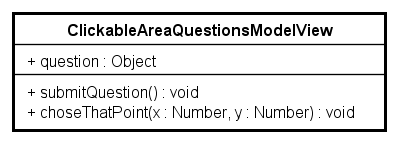
\includegraphics[scale=0.80]{UML/Classi/Front-End/QuizziPedia_Front-end_ModelView_ClickableAreaQuestionsModelView.png}
	\caption{QuizziPedia::Front-End::ModelViews::ClickableAreaQuestionsModelView}
\end{figure} \FloatBarrier
\begin{itemize}
	\item \textbf{Descrizione}: classe di tipo modelview la cui istanziazione è contenuta all'interno della variabile di ambiente \texttt{\$scope} di \textit{Angular\ped{G}}. All'interno di essa sono presenti le variabili e i metodi necessari per il \textit{Two-Way Data-Binding\ped{G}} tra la \textit{view\ped{G}} \texttt{ClickableAreaQuestionsView} e il \textit{controller\ped{G}} \texttt{ClickableAreaQuestionsController}; 
	\item \textbf{Utilizzo}: viene utilizzata per effettuare il \textit{Two-Way Data-Binding\ped{G}} tra la \textit{view\ped{G}}\\ \texttt{ClickableAreaQuestionsView} e il \textit{controller\ped{G}} \texttt{ClickableAreaQuestionsController} rendendo disponibili variabili e metodi;
	\item \textbf{Relazioni con altre classi}:
	\begin{itemize}
		\item \textbf{IN \texttt{ClickableAreaQuestionsView}}: \textit{view\ped{G}} contenente i campi e le direttive per creare una domanda ad area cliccabile; 
		\item \textbf{IN \texttt{ClickableAreaQuestionsController}}: questa classe permette di gestire la creazione e la modifica di una domanda ad area cliccabile.
	\end{itemize}
	\item \textbf{Attributi}:
	\begin{itemize}
			\item \texttt{+ question: Object} \\ Oggetto contenente gli attributi per la creazione della domanda:
			\begin{itemize}
				\item \texttt{url: String}: attributo di tipo \texttt{String} che contiene l'\textit{URL\ped{G}} associato all'immagine;
				\item \texttt{answer: Array}: array contenente oggetti che rappresentano le risposte. Ogni oggetto risposta contiene:
				\begin{itemize}
					\item \texttt{x: Number}: attributo di tipo \texttt{Number} che rappresenta la posizione della risposta nell'asse delle ascisse all'interno dell'immagine;
					\item \texttt{y: Number}: attributo di tipo \texttt{Number} che rappresenta la posizione della risposta nell'asse delle ordinate all'interno dell'immagine.
				\end{itemize}
	\end{itemize}
	\item \textbf{Metodi}:
	\begin{itemize}
			\item \texttt{+ submitQuestion(): void}\\ 
			Metodo che gestisce l’evento click sul pulsante di conferma sulla domanda. Raccoglie i dati dal modelview e li manda al server attraverso \texttt{QuestionService}. Poi verrà effettuato il redirect alla pagina di gestione delle domande oppure al questionario che si stava creando; 
			\item \texttt{+ choseThatPoint(x: Number, y: Number): void}\\
			Metodo che gestisce l’evento click su un punto dell'immagine. Una volta selezionato esso verrà inserito nell'array di punti. \\
			\textbf{Parametri}:
			\begin{itemize}
				\item \texttt{x: Number} \\
				Parametro contenente la coordinata x del punto;
				\item \texttt{y: Number} \\ 
				Parametro contenente la coordinata y del punto.
			\end{itemize}
	\end{itemize}
\end{itemize}
\end{itemize}

